\section{Experiments}
\label{sec:Exp}

\subsection{Training strategies}
\label{sec:ExpStra}

The approach of this study is implemented by 
the open source framework PyTorch. 
\cite{Abadi2016}
The pre-trained models for initializing the 
network parameters are acquired from 
torchvision.
\cite{Paszke2017}
Models are trained and tested on a graphic 
workstation with an Intel Core i9-7980XE 
CPU(2.60 GHz, 18 core) and a GeForce GTX 
1080Ti GPU. As described in 
Section~\ref{sec:Data}, 
we choose a dataset DDSM to train and test 
our proposed network in the experiments. 

In the training phase, we use a stochastic 
gradient descent method with a batch size of 32, 
\cite{Ioffe2015}
a momentum of 0.9 and a weight decay of 
0.0005 similar to optimize our models 
for 100 epochs. As shown in 
Figure~\ref{fig:extrFusion}, 
we propose a method fusing 3 models with 
similar structure and freezing different 
layers called Freeze1 to Freeze3 from top to 
bottom. The accuracy curves on the 
validation dataset of 3 models in the 
training phase are shown in 
Figure~\ref{fig:resAcc}. 
Due to the warmup strategy,
\cite{Glorot2011}
the accuracy grows 
slowly in the first 5 epochs. A relatively 
large batch size reduces the noise in the 
gradient, and an increased learning rate 
can make a larger progress along the 
opposite of the gradient direction.
\cite{Liu2020}
Since our network structure is based on 
DenseNet, the learning rate is initialized to 
0.01 and lowered by 10 times every 20 
epochs in the experiments.
\cite{Jia2014}

\begin{figure*}[!ht]
    \centering
    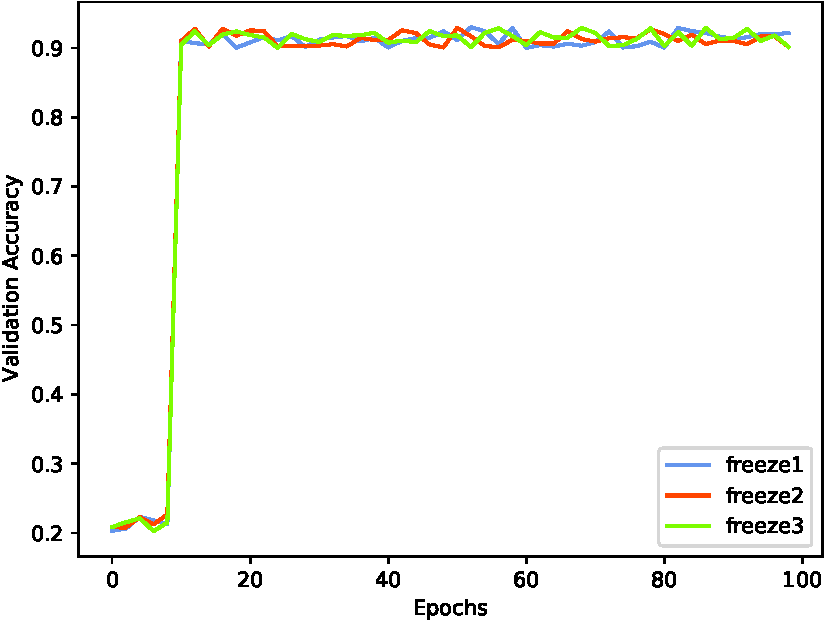
\includegraphics[
        width=0.6\textwidth,
        keepaspectratio
    ]{acc.pdf}
    \caption{Validation accuracy.}
    \label{fig:resAcc}
\end{figure*}

Although the parameters of the network 
were initialized with the model trained by 
ImageNet at the beginning of the training 
phase, and the model is far from the final 
solution, we adopt a warmup strategy by using 
a very small learning rate 0.00001 in the 
first 5 epochs and then switch to the 
initial learning rate when the training 
process is stable. Besides, for every 5 
epochs, we compare the performance between 
the current model and the best model of 
previous epochs. If the previous one 
performs better, the parameters in the 
former model will be loaded into the 
current model before the next epoch starts.

\subsection{Results}
\label{sec:ExpRes}

For mammography image recognition, the DDSM 
dataset contains 753 calcification cases, 
providing a data-set size capable of 
analyzing decision support systems in 
mammography. We also compared the results 
on the DDSM dataset with other methods 
including CNN feature-based methods. 
As shown in 
Table~\ref{tab:tabPerf},
the proposed method achieved high accuracy 
close to other methods without obvious 
advantages on the DDSM dataset. We also trained 
3 models concentrating on different kind
of features by freezing different 
parameters during training. This method 
performs better on a fine-grained 
classification task. Our method achieved 
high accuracy on this task, significantly 
higher than other methods.

\begin{table*}[!ht]
    \caption{Performance comparing to 
        different methods}
    \label{tab:tabPerf}
    \setlength{\arrayrulewidth}{1.05 pt}
    \renewcommand{\arraystretch}{1.1}
    \begin{tabular*}{1.0\textwidth}{
        @{
            \extracolsep{\fill}
        }ll
    }
        \hline
        Method & Accuracy($\%$) \\
        \hline
        SIFT-BoVW       & 89.05 \\
        VGGNet          & 90.01 \\
        AGNet           & 91.28 \\
        Inception       & 93.48 \\
        DenseNet        & 93.70 \\
        Our             & 94.68 \\
        \hline
    \end{tabular*}
\end{table*}

\subsection{Statistical analysis of fusion method}
\label{ExpSA}

In the previous sections, we have proposed 
a method which fuses 3 models with different 
layers’ parameters frozen to improve 
performance, particularly in 
Section~\ref{sec:MethNetFea} 
we mention that different models 
concentrate on different aspects of input 
images. To evaluate the diversity of 3 
models, we conduct statistical analysis with 
a series of ablation studies.

Firstly, we try to fuse any 2 models of 3 
models with different frozen parameters and 
calculate their accuracies on the test set 
comparing to a single model. Details of
the results are listed in 
Table~\ref{tab:tabFusionAny2}. 
F1–F4 represent model Freeze1 to Freeze4 
respectively and \& means fusing two
models together, for instance, F1\&F2 
means fusing model Freeze1 and Freeze2. 
According to the results, we find that 
fusing any of 2 models always performs 
better than a single one for each category. 
It can be concluded that models with 
different layers’ parameters frozen focus 
on different features of images in different 
categories, which leads to the fused network 
model get better performance.

\begin{table*}[!ht]
    \caption{Results of fusing any 2 models}
    \label{tab:tabFusionAny2}
    \setlength{\arrayrulewidth}{1.05 pt}
    \renewcommand{\arraystretch}{1.1}
    \begin{tabular*}{1.0\textwidth}{
        @{
            \extracolsep{\fill}
        }lcccccc
    }
        \hline
        
        Category & F1($\%$) & F2($\%$) & F3($\%$) 
        & F1$\&$F2($\%$) 
        & F1$\&$F3($\%$)  
        & F2$\&$F3($\%$)  \\
        
        \hline
        
        1 & 90.55 & 89.60 & 92.06 
        & 92.30 & 93.05 & 93.05 \\
        
        2 & 89.03 & 91.13 & 93.37 
        & 92.08 & 96.02 & 97.06 \\
        
        3 & 90.37 & 93.02 & 91.07 
        & 93.51 & 93.60 & 94.05 \\
        
        4 & 88.70 & 88.67 & 89.06 
        & 92.07 & 93.05 & 94.08 \\
        
        5 & 89.50 & 89.60 & 90.05 
        & 92.30 & 94.70 & 95.05 \\
        
        6 & 92.06 & 89.09 & 94.06 
        & 91.03 & 94.03 & 97.04 \\
        
        7 & 91.05 & 89.60 & 92.06 
        & 92.30 & 93.05 & 96.02 \\
        
        \hline
    \end{tabular*}
\end{table*}

In addition, when testing each single 
network’s performance, we count the numbers 
of instances that only one model recognizes 
them wrongly while the other three predict 
correctly. As shown in columns from 3 to 6 
in Table~\ref{tab:tabFusionAny1}, 3 models 
don’t give the same predicting result of
every image in each category. For each 
category, there are dozens of images which 
recognized wrongly by only one model, 
and the other 2 models can recognize them 
better.

\begin{table*}[!ht]
    \caption{Comparison of number of images 
        recognized wrongly by only one model}
    \label{tab:tabFusionAny1}
    \setlength{\arrayrulewidth}{1.05 pt}
    \renewcommand{\arraystretch}{1.1}
    \begin{tabular*}{1.0\textwidth}{
        @{
            \extracolsep{\fill}
        }lccccc
    }
        \hline
        
        Category & Total & Freeze1 & Freeze2 
        & Freeze3 & All \\
        
        \hline
        
        1 & 1172 & 58 & 44 & 31 & 0 \\
        2 & 1029 & 24 & 29 & 36 & 0 \\
        3 & 1105 & 36 & 61 & 44 & 0 \\
        4 &  859 & 48 & 41 & 56 & 0 \\
        5 &  786 & 76 & 87 & 36 & 0 \\
        6 &  907 & 15 & 29 & 41 & 0 \\
        7 &  937 & 80 & 29 & 64 & 0 \\
        
        \hline
    \end{tabular*}
\end{table*}

And It can be observed that none of the images 
are wrongly recognized by all the 3 models 
at the same time, from the last column in 
Table~\ref{tab:tabFusionAny1}. 
In other words, the 3 models pay attention 
to different aspects of the images, and each 
model has its advantage and drawback.
By integrating them and fusing their 
extracted diversified features together, 
the ensemble model learns more 
representative features.

\subsection{Analysis the hash decoder}
\label{ExpHash}

In this work, one of the innovation points, is to 
employ a hash decoder to reduce the difficulty
of computing the high dimenision parameters. A 
natural alternative to the hash decoder is
a simple fully-connected layer followed by 
a sigmoid layer of restricting the output 
values’ range in [0, 1]. To investigate the 
effectiveness of the hash decoder. Implement 
and evaluate a single deep network-based
DenseNet, connecting with its alternative
choice which is a fully network. In the end,
we employe a single classifier based SVM. To
do this, to prove our hash decoder is 
effective. As can be seen from 
Table~\ref{tab:tabHash}, 
the results of the proposed method outperform 
the competitor with the alternative. For 
example, the architecture with hash decoder 
achieves the accuracy of 0.581 with 48 bits, which 
indicates an improvement of 19.7$\%$ over the 
FC alternative. The underlying reason for
the improvement may be that, compared to the 
FC alternative, the output hash codes from 
the hash decoder are less redundant to each 
other.

\begin{table*}[!ht]
    \caption{Comparison results of the hash 
        decoder and fully connection}
    \label{tab:tabHash}
    \setlength{\arrayrulewidth}{1.05 pt}
    \renewcommand{\arraystretch}{1.1}
    \begin{tabular*}{1.0\textwidth}{
        @{
            \extracolsep{\fill}
        }lllll
    }
        \hline
        
        Method(MAP) & 12 bits & 24 bits & 32 bits & 48 bits \\
                
        \hline

        FC    & 0.877 & 0.896 & 0.909 & 0.912 \\       
        Ours  & 0.899 & 0.914 & 0.925 & 0.923 \\
        
        \hline
    \end{tabular*}
\end{table*}

\subsection{Comparing to the single classifier}
\label{ExpCls}

To investigate the effectiveness of the fusion
of the classifiers. A single DenseNet is employed
for this experiment, beacause it can maintain 
the invariance of the feature vector and enlarging 
the impact of classifier differences on test 
results. The specific 
experimental results are shown in the 
Table~\ref{tab:tabCls}. From the data in the 
table, we can see that the difference between 
different classifiers is more obvious, and 
the effect of random forest is better, but 
the result of the fused classifier is the best. 
The reason for this is that the principle of 
different classifiers is different and the 
sensitivity of features is different. It is 
obvious that the results of the fusion 
classifier can make the accuracy more reliable.

\begin{table*}[!ht]
    \caption{Comparison results of the 
        classifers}
    \label{tab:tabCls}
    \setlength{\arrayrulewidth}{1.05 pt}
    \renewcommand{\arraystretch}{1.1}
    \begin{tabular*}{1.0\textwidth}{
        @{
            \extracolsep{\fill}
        }ll
    }
        \hline
        
        Classifier & Accuracy($\%$) \\
                
        \hline

        k-NN            & 83.50 \\ 
        SVM             & 85.70 \\ 
        RandomForest    & 87.09 \\ 
        Ours            & 91.49 \\
        
        \hline
    \end{tabular*}
\end{table*}

\subsection{Comparing to single network methods}
\label{ExpCS}

There have been approaches with single 
network structures applied on DDSM,
well-performed structures like VGGNet, 
Inception, ResNet and etc are used as 
the backbones for constructing the networks 
of mammography image recognition approaches. 
To figure out which backbone is most suitable
for this task, the experiments are conducted 
to test the performance of the network with 
different backbones. 
Figure~\ref{fig:resAccDiff} shows the 
accuracy of several backbones we tried on the 
validation set during 100 training epochs. 
In the first 5 epochs, the accuracy grows 
slowly because of the warmup strategy 
mentioned in Section~\ref{sec:ExpStra}, 
and the learning rate is set to a 
relatively small value before the training 
process is stable. We found the accuracy of 
DenseNet is slightly higher than other mod-
els in the experiment. Hence it is used as 
one of the backbones.

\begin{figure*}[!ht]
    \centering
    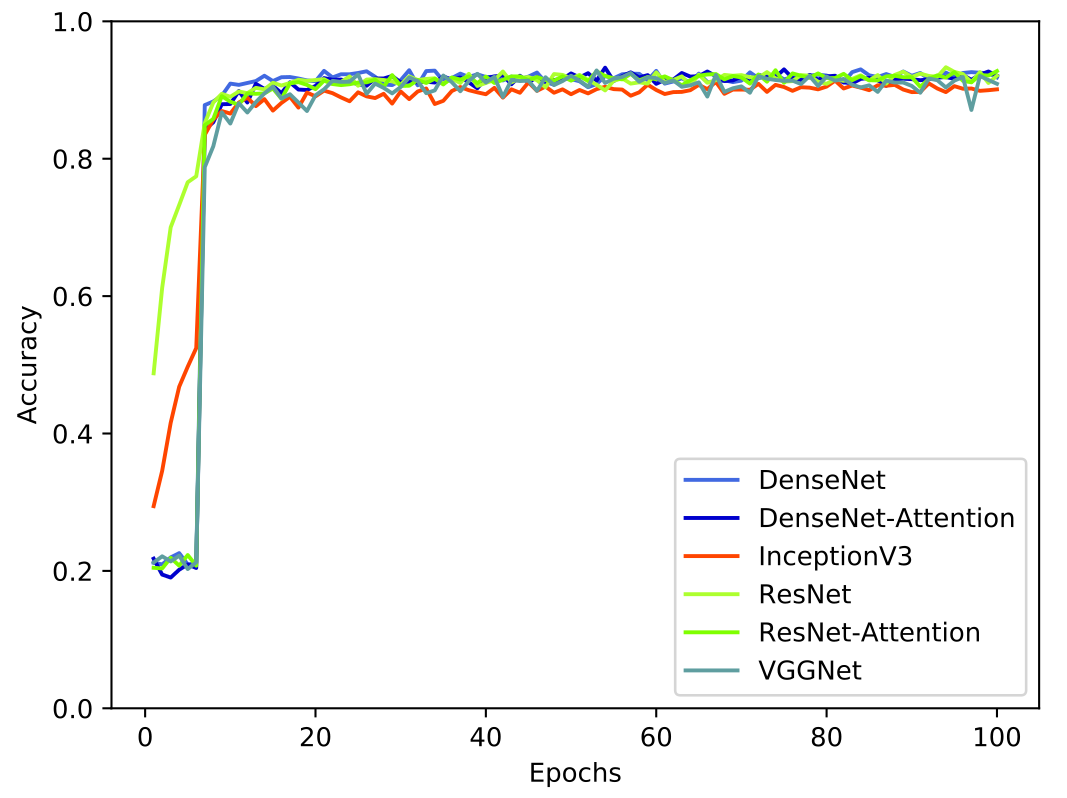
\includegraphics[
        width=0.6\textwidth,
        keepaspectratio
    ]{acc_back.png}
    \caption{Validation accuracy of different 
        backbone.}
    \label{fig:resAccDiff}
\end{figure*} 

The proposed transfer learning model 
fusion method is shown in 
Figure~\ref{fig:extrFusion}, 
3 models are trained in parallel with 
different frozen parameters. weight of each 
model is set manually according to the 
singles model’s accuracy. The accuracy of 
each single model with different frozen 
parameters is shown in 
Table~\ref{tab:tabFusionPara}. 
For instance, model Freeze1 represents the 
top row in 
Figure~\ref{fig:extrFusion}, 
which is the model with the most frozen 
parameters. In our work, 
we test different weights for each model 
according to their accuracies on the 
validation set, as shown in 
Figure~\ref{fig:resAcc}. 
Lastly, the weights 
for 3 models are set to [0.4, 0.4, 0.3].

\subsection{Comparing different network fusion 
    methods}
\label{ExpCD}

\begin{figure*}[!ht]
    \centering
    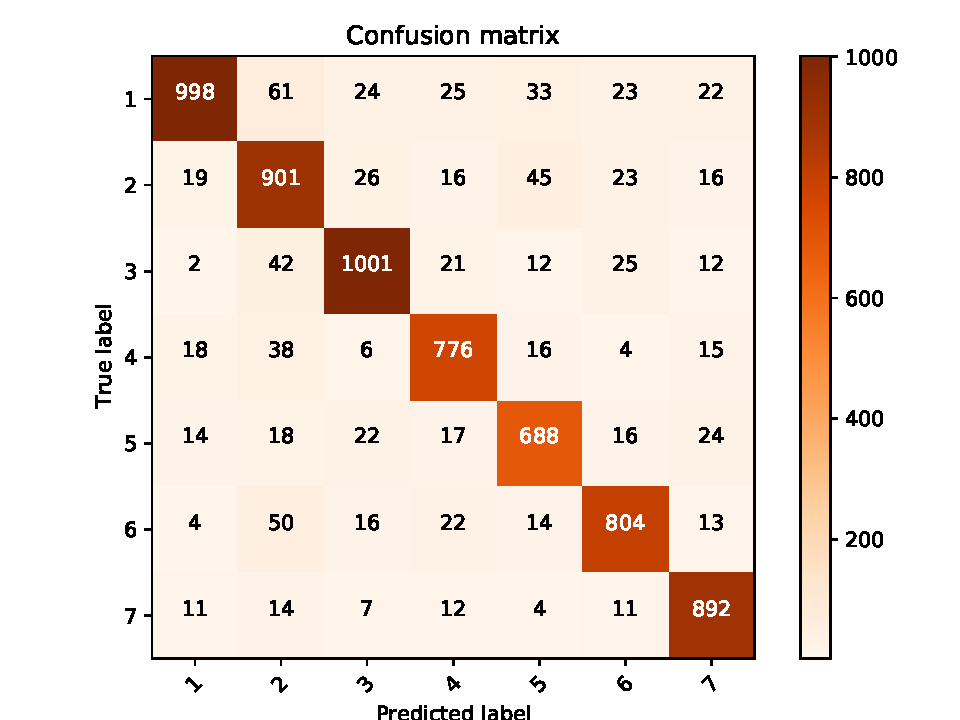
\includegraphics[
        width=0.49\textwidth,
        keepaspectratio
    ]{nonnorm_f1.pdf}
    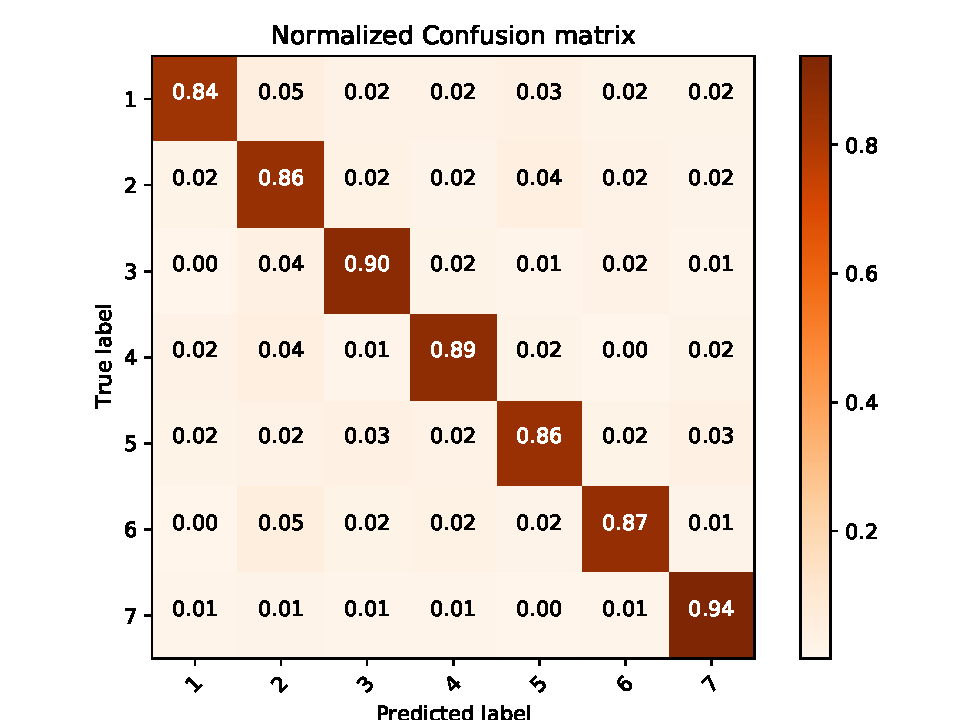
\includegraphics[
        width=0.49\textwidth,
        keepaspectratio
    ]{norm_f1.pdf}
    \caption{Confusion matrices produced by the 
        first frozen models on the test set}
    \label{fig:resFreeze1}
\end{figure*}   

\begin{figure*}[!ht]
    \centering
    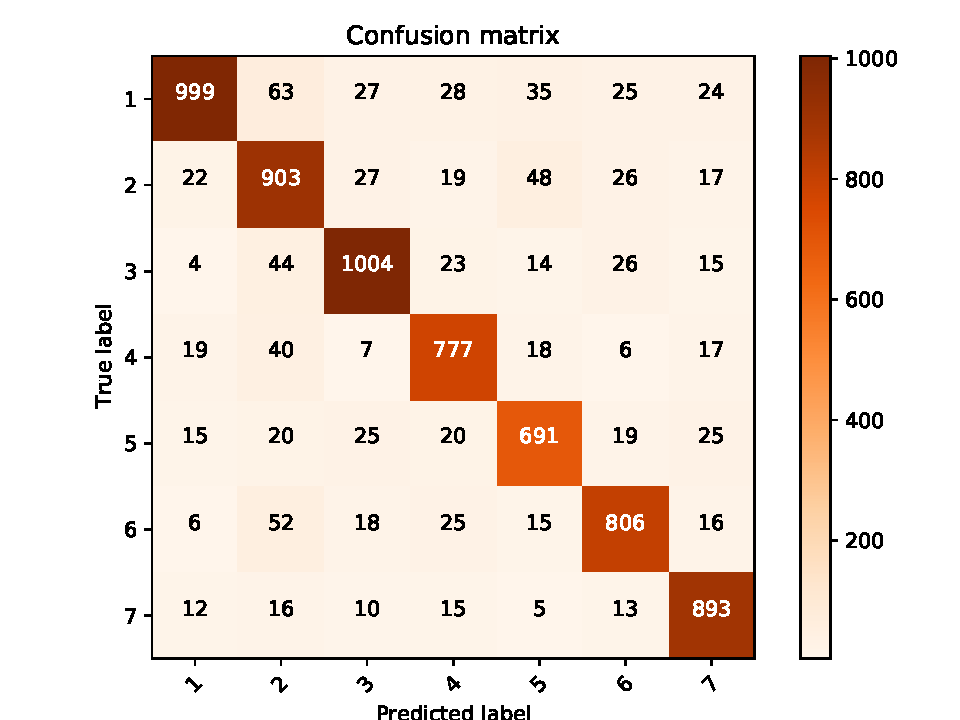
\includegraphics[
        width=0.49\textwidth,
        keepaspectratio
    ]{nonnorm_f2.pdf}
    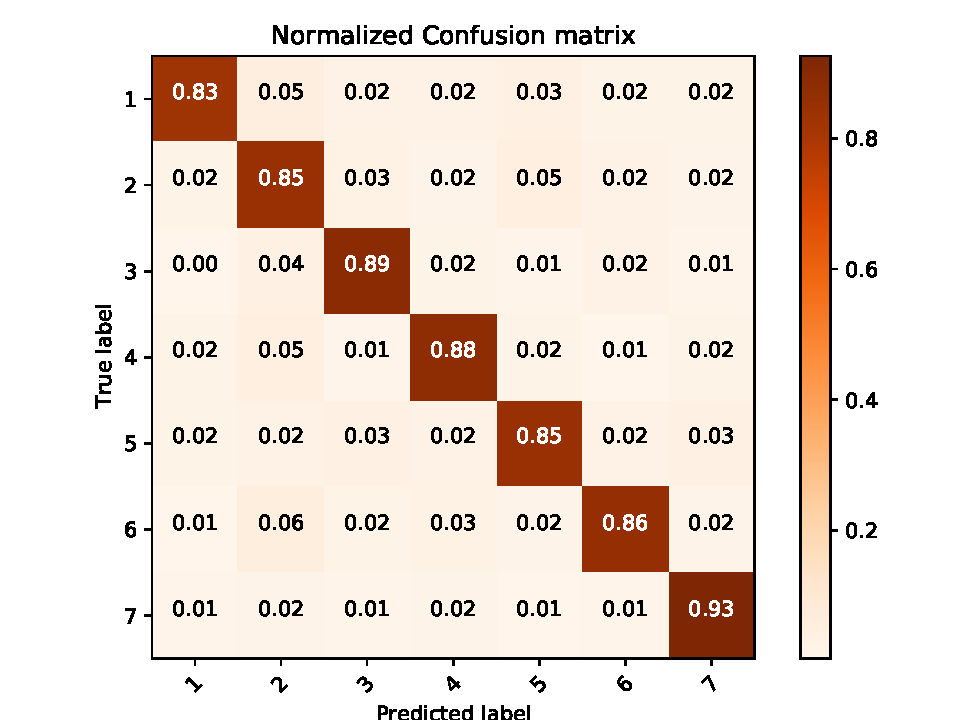
\includegraphics[
        width=0.49\textwidth,
        keepaspectratio
    ]{norm_f2.pdf}
    \caption{Confusion matrices produced by the 
        second frozen models on the test set}
    \label{fig:resFreeze2}
\end{figure*} 

\begin{figure*}[!ht]
    \centering
    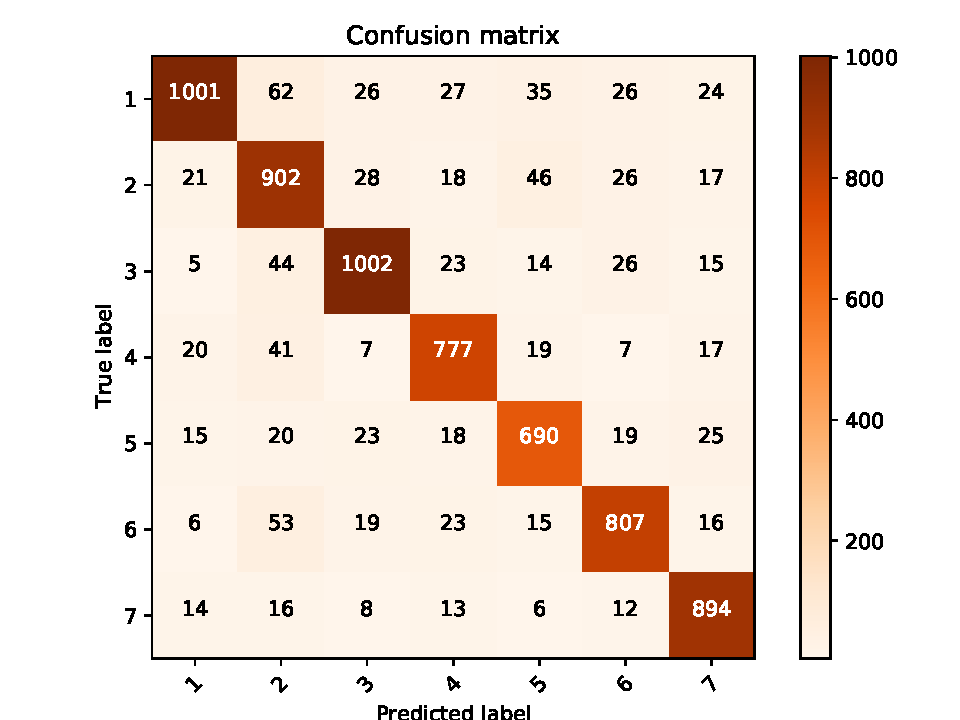
\includegraphics[
        width=0.49\textwidth,
        keepaspectratio
    ]{nonnorm_f3.pdf}
    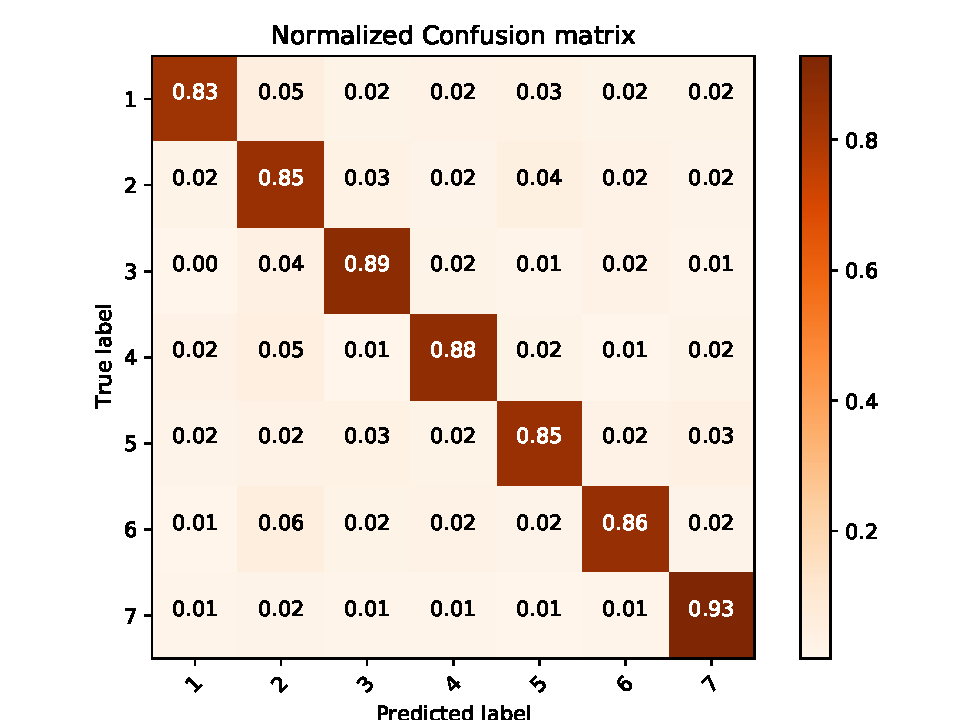
\includegraphics[
        width=0.49\textwidth,
        keepaspectratio
    ]{norm_f3.pdf}
    \caption{Confusion matrices produced by the 
        thirty frozen models on the test set}
    \label{fig:resFreeze3}
\end{figure*} 

\begin{table*}[!ht]
    \caption{Comparing with the single network 
        based methods on DDSM dataset}
    \label{tab:tabFusionNet}
    \setlength{\arrayrulewidth}{1.05 pt}
    \renewcommand{\arraystretch}{1.1}
    \begin{tabular*}{1.0\textwidth}{
        @{
            \extracolsep{\fill}
        }lll
    }
        \hline
        
        Method & Accuracy($\%$) 
        & Average inference time (ms) \\
        
        \hline
        
        VGGNet based        & 90.09 & 6.062 \\
        InceptionV3 based   & 92.16 & 2.396 \\
        ResNet50 based      & 93.08 & 3.006 \\
        DenseNet based      & 92.67 & 3.762 \\
        Our                 & 94.48 & 15.052 \\
        
        \hline
    \end{tabular*}
\end{table*}

We have proposed a method of fusing 3 models 
with different network structure but different 
frozen parameters. This idea is inspired by AGNet, 
a method enriching extracted features by combining 
2 networks with a weighted sum. Due to the 
different topological structures, the relationship
between features they extracted is relatively weak 
and we cannot assure that they have learned 
knowledge of different aspects from the training 
images.

\begin{table*}[!ht]
    \caption{Accuracies of models with different 
        parameters frozen}
    \label{tab:tabFusionPara}
    \setlength{\arrayrulewidth}{1.05 pt}
    \renewcommand{\arraystretch}{1.1}
    \begin{tabular*}{1.0\textwidth}{
        @{
            \extracolsep{\fill}
        }lll
    }
        \hline
        
        Models & Freeze params & Test accuracy($\%$) \\
        
        \hline
        
        Freeze1 & 4.76M & 93.01 \\
        Freeze2 & 3.50M & 92.36 \\
        Freeze3 & 0.95M & 91.88 \\
        Fusion  &  -    & 94.48 \\
        
        \hline
    \end{tabular*}
\end{table*}

In the experiments, we test the methods of 
fusing models in different network structures 
and on the DDSM dataset. As shown in 
Figure~\ref{fig:resFreeze1} to 
Figure~\ref{fig:resFreeze3}, 
among the 3 models we trained, Freeze3 
achieves the best result on the validation set 
during the training phase. Therefore, we try 
to fuse it with other models in different 
network structure such as VGGNet, Inception,
ResNet to check whether the fusion models 
in different network structure helps improve 
the performance or not. The parameters of 
these models are initialized by the 
corresponding pre-trained model on ImageNet 
and their shallow layers are frozen while 
training. According to the results listed in
Table~\ref{tab:tabFusionNet}, 
compared to the single network-based method, 
it has higher accuracy, but fusing 3 models 
still performs better. In this way, the 
network extracts more rich features and the 
classifier produces better recognition 
results.

\begin{figure*}[!ht]
    \centering
    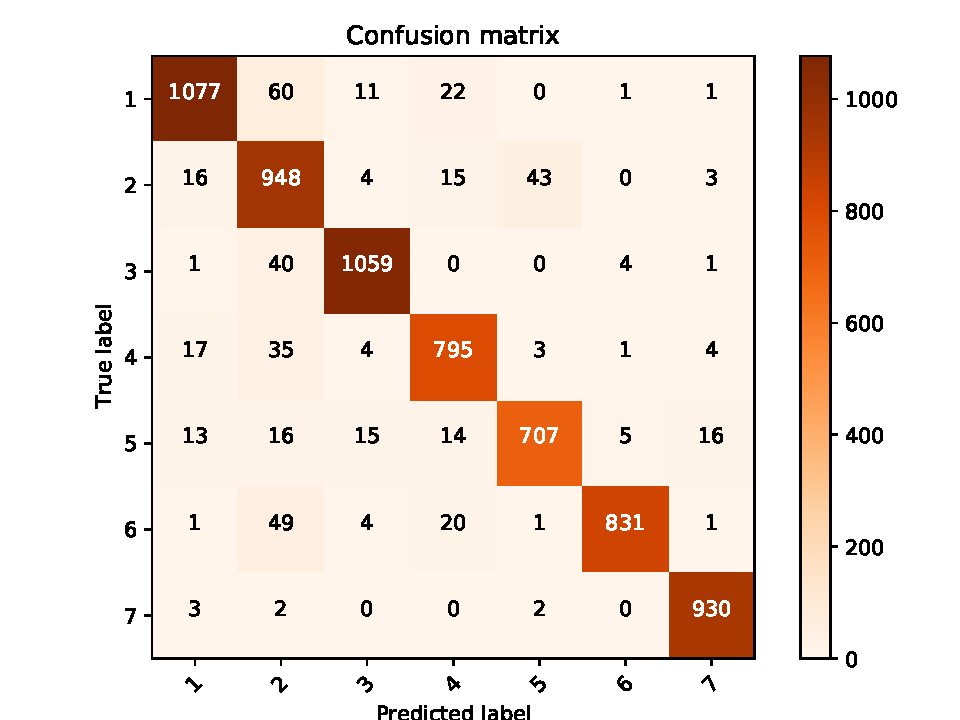
\includegraphics[
        width=0.49\textwidth,
        keepaspectratio
    ]{nonnorm.pdf}
    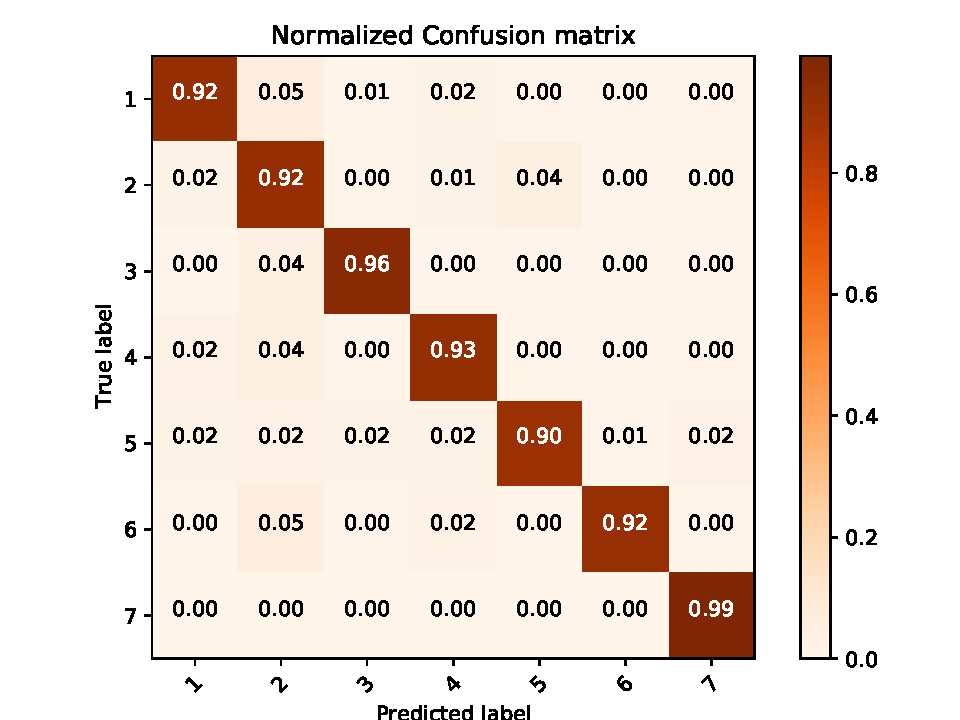
\includegraphics[
        width=0.49\textwidth,
        keepaspectratio
    ]{norm.pdf}
    \caption{Confusion matrices produced by the 
        fusion model on the test set.}
    \label{fig:resFusionMat}
\end{figure*}

Figure~\ref{fig:resFusionMat} 
shows the classification results of each 
class with confusion matrix. The accuracies 
of 7 classes are higher than 92$\%$. Because 
the features are learned from the training 
set and there are some overlapping image 
parts between classes, which contain a large 
images are more likely be wrongly classified.

\subsection{Comparing other object detection methods}
\label{ExpCD}

For the target detection module of this 
work, it is mainly based on the Faster RCNN 
framework, and the innovation of this study 
is also the innovation of the classification 
stage. For the object detection module, we 
made a simple comparison with the original 
framework model in terms of time and 
accuracy. The specific experimental results 
are shown in 
Table~\ref{tab:tabOD}. 
It is obvious from the data in the table 
that our method greatly improves the 
calculation time of the model without 
losing accuracy. Combining with our model 
framework, the reason can be clearly found 
because we have introduced a hash recoder 
module.

\begin{table*}[!ht]
    \caption{Comparing to the region RCNN}
    \label{tab:tabOD}
    \setlength{\arrayrulewidth}{1.05 pt}
    \renewcommand{\arraystretch}{1.1}
    \begin{tabular*}{1.0\textwidth}{
        @{
            \extracolsep{\fill}
        }lll
    }
        \hline
        
        Models & mAP($\%$) & time(ms) \\
        
        \hline
        
        Fast RCNN   & 60.50 & 534 \\
        Faster RCNN & 70.03 & 325 \\
        Ours        & 75.01 & 105 \\

        \hline
    \end{tabular*}
\end{table*}
